% VERSION: 1.0.0
\documentclass[letterpaper, 10 pt, conference]{ieeeconf}

\IEEEoverridecommandlockouts  % use the \thanks command
\overrideIEEEmargins % See \addtolength -- to balance the column lengths on the last page of the document

\usepackage[utf8]{inputenc}
\usepackage[T1]{fontenc}

% Other useful packages:
\usepackage{graphics} % for pdf, bitmapped graphics files
% \usepackage{amsmath}
\usepackage{algorithm}
\usepackage[noend]{algpseudocode}
% \usepackage{lscape}
\usepackage[paper=portrait,pagesize]{typearea}

\usepackage[backend=bibtex,sorting=none]{biblatex}
\bibliography{Software-Problems-2022}


\title{\LARGE \bf
Comparing Applications with the Software Problem Area Taxonomy
}

%%%%%%%%%%%%%%%%%%%%%%%%%%%%%%%%%%%%%%%%%%%%%%%%%%%%%%%%%%%%%%%%%%%%%%%%%%%%%%%%
\author{
  \parbox{2.0 in}{\centering Maj Brandon Froberg}
  \hspace{ 0.15 in}
  \parbox{2.0 in}{ \centering MSgt Erik Olson}
  \hspace{ 0.15 in}
  \parbox{2.0 in}{ \centering Mr. Duane Baldish}
}
%%%%%%%%%%%%%%%%%%%%%%%%%%%%%%%%%%%%%%%%%%%%%%%%%%%%%%%%%%%%%%%%%%%%%%%%%%%%%%%%

\begin{document}
\maketitle
\thispagestyle{empty}
\pagestyle{empty}


%%%%%%%%%%%%%%%%%%%%%%%%%%%%%%%%%%%%%%%%%%%%%%%%%%%%%%%%%%%%%%%%%%%%%%%%%%%%%%%%
% ABSTRACT
\begin{abstract}

There are numerous methods and models to type, classify, describe, and compare software applications.
Yet, there is a lack of software taxonomies, which categories software applications in terms of problems and solution spaces.
We created a software problem taxonomy for use within Air Force Special Operations Command (AFSOC).
The novel taxonomy enables comparing and contrasting software applications, but specifically focuses on the problems the software applications aim to solve.
Our approach enables more fair comparisons of applications to solve or fulfill requirements and/or capability gaps.
  
\end{abstract}
%%%%%%%%%%%%%%%%%%%%%%%%%%%%%%%%%%%%%%%%%%%%%%%%%%%%%%%%%%%%%%%%%%%%%%%%%%%%%%%%


%%%%%%%%%%%%%%%%%%%%%%%%%%%%%%%%%%%%%%%%%%%%%%%%%%%%%%%%%%%%%%%%%%%%%%%%%%%%%%%%
\section{BACKGROUND}
%
%
AFSOC, and the Department of Defense writ large, has capability gap to accurately compare and contrast available software solutions via the problems they solve.
Situations arise in which software applications are directly compared by using descriptive attributes (e.g., a categorization of career/functional area, or development method).
Often, comparisons of attributes are irrelevant, because they fail to consider the problem space first.
For instance, "Enterprise Level" solutions are treated as a one size fits all application based only on descriptive attributes.
Fair comparisons should first consider the problem space the software application is used to solve.
%%%%%%%%%%%%%%%%%%%%%%%%%%%%%%%%%%%%%%%%%%%%%%%%%%%%%%%%%%%%%%%%%%%%%%%%%%%%%%%%


%%%%%%%%%%%%%%%%%%%%%%%%%%%%%%%%%%%%%%%%%%%%%%%%%%%%%%%%%%%%%%%%%%%%%%%%%%%%%%%%
\section{RESEARCHING EXISTING TAXONOMIES}
%
%
In our initial research, we did not encounter software classifying methods/models which considered problem spaces.
Existing software classifications methods/models use descriptive attributes to type, classify, describe application capabilities.
For instance, the seminal Forward \& Lethbridge taxonomy is robust, but we feel it focuses on software capabilities and/or descriptive attributes\cite{forward2008taxonomy}.
We argue the taxonomy classifies software by implementations of tools, techniques, or procedures; thus, we created a method to classify software by the problems they solve:

%see: https://tex.stackexchange.com/questions/163768/write-pseudo-code-in-latex
\begin{algorithm}
  \caption{Classifying Software by Problems}\label{euclid}
  \begin{algorithmic}[1]
  \Procedure{Mapping Sofware to Problem Space}{}
  \State $\textit{\bf A} \gets $\textit{software application/capabilities}
  \State $\textit{\bf B} \gets $\textit{problem space category/sub-category}
  \State $\textit{An } $\textit{\bf A} $\textit{is used to solve a problem in } $\textit{\bf B}
  \EndProcedure
  \end{algorithmic}
\end{algorithm}

Comparatively, Forward \& Lethbridge's taxonomy follows a method which mapped software into a domain of \textbf{A} (i.e., software capabilities) versus \textbf{B} (i.e., a problem space).
 
For example: A \textbf{decision support system} (A.bus.3) or \textbf{inventory control} (D.im.1) app is used to solve problem in \textbf{Data Analysis} and \textbf{Data Visualization}.
Other research or taxonomies for software categorization showed a similar lack of describing apps by their respective problem spaces\cite{capiluppi2020towards}\cite{villalon2015taxonomy}\cite{barnes2013software}\cite{kasunic2008data}\cite{usman2015supporting}\cite{stray2020agile}.
%%%%%%%%%%%%%%%%%%%%%%%%%%%%%%%%%%%%%%%%%%%%%%%%%%%%%%%%%%%%%%%%%%%%%%%%%%%%%%%%


%%%%%%%%%%%%%%%%%%%%%%%%%%%%%%%%%%%%%%%%%%%%%%%%%%%%%%%%%%%%%%%%%%%%%%%%%%%%%%%%
\section{Creating a "16th Standard"}
%
%

Randall Monroe, the author of xkcd comics, presents a satire on how standards proliferate:


\begin{figure}[h]
  \centering
  \scalebox{.4}{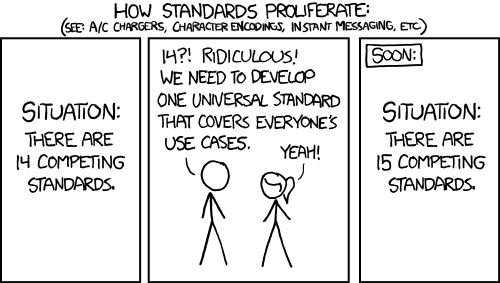
\includegraphics{./images/standards.png}}
  \caption{XKCD's "Standards"\cite{munroe927}}
\end{figure}

Given the absence of software taxonomies, which focus on software problem spaces, we propose the Software Problem Area Taxonomy (SPAT):

\begin{table}[h]
\begin{center}
\begin{tabular}{|c||c|}
\hline
\bf Main Category & \bf Sub-Category\\
\hline
Business Software & Presentation, Word Processing,  \\
& \newline Mathematical Spreadsheets\\
\hline
Computer Management & Command \& Control (C2),\\
& \newline Remote Access, Patching \& Updates,\\
& \newline Device Management\\
\hline
Data Analysis & Manual, Automatic, \\
& \newline  Machine Learning-based, AI-based\\
\hline
Data Collection & Primary, Secondary+, Archival\\
\hline
Digital Assembly & Drafting, Manufacturing,\\
& \newline Multimedia, Visualization \\
\hline
Information Transfer & Audio, Video, Text, Raw\\
\hline
Information Visualization & Dashboarding, Summary\\
\hline
Modeling \& Simulation & Manual, Automatic,\\
& \newline  Model Generation/Refinement,\\
& \newline  Visualization, Wargaming\\
\hline
Workflow \& Processing & Manual, Automatic\\
& \newline  Non-repudiation Receipt\\
\hline
\end{tabular}
\end{center}
\caption{A Subset of SPAT Version 0.1.0 Categories}
\label{}
\end{table}

We present version 0.1.0, using Semantic Versioning to describe Major, Minor, and Patch releases.
Our proposition is not an all-encompassing list.
Also, we fully expect the main and sub categories to expand, and undergo further refinement, as the larger Department of Defense and industry partners communities review this taxonomy.
 
 
Another important consideration to the taxonomy is to enable, capture, and describe software in terms of metadata attributes.
Attributes are largely captured in existing taxonomies, inclusion further extends the qualification of application taxonomy mapping.
Joining the problem space category to applicable attributes gives broader capabilities to sort, type, and categorize apps.
For instance Data Analysis and Information Visualization categories may contain Aircraft Logistical Supply and Computer Logistics Management apps, yet including metadata attributes permits a differentiatiion of the apps.
Thus, the developed taxonomy includes collecting metadata attributes, and a subset is shown below:

\begin{table}[h]
\begin{center}
\begin{tabular}{|c||c|}
\hline
\bf Attribute & \bf Example Descriptor\\
\hline
Development Technique & Traditional, Agile, DevSecOps Pipeline\\
\hline
Security & Manual, Automatic, \\
& \newline  Machine Learning-based, AI-based\\
\hline
Functional Area & Mission Planning, C2\\
& \newline Communications, Computers, \\
& \newline Financial, Acquisition, Development, \\
& \newline Intelligence, Surveillance, Reconnaissance\\
\hline
Code Level & Low Level/Binary, Bytecode, \\
& \newline Intermediate representation, Script, \\
& \newline No-code\\
\hline
Rendering & 2D, 3D, Augmented\\
\hline
\end{tabular}
\end{center}
\caption{Example Software Application Metadata Attributes}
\label{}
\end{table}

%%%%%%%%%%%%%%%%%%%%%%%%%%%%%%%%%%%%%%%%%%%%%%%%%%%%%%%%%%%%%%%%%%%%%%%%%%%%%%%%

%%%%%%%%%%%%%%%%%%%%%%%%%%%%%%%%%%%%%%%%%%%%%%%%%%%%%%%%%%%%%%%%%%%%%%%%%%%%%%%%
\section{USING THE TAXONOMY}
%
%
Currently the taxonomy is used for immediate comparisons in Analysis of Alternatives and In-progress Reviews within the AFSOC Headquarters.
We have several application comparisons that are in progress.
The main comparison is of Robotic Process Automation (RPA) tools.
Using our taxonomy shows how RPA tools are not one-to-one.
Moreover, the taxonomy enables a clear and separate comparison of tools that can directly be used to justify funding and project continuation and/or support.

Additionally, AFSOC has an education \& training initiative which enables and empowers citizen developers in the command.
Our taxonomy is being used as an education tool to assist our trainees while they draft capability/business needs statements.
This education facilitates the identification of requirements and essential capabilities prior to application development.
%%%%%%%%%%%%%%%%%%%%%%%%%%%%%%%%%%%%%%%%%%%%%%%%%%%%%%%%%%%%%%%%%%%%%%%%%%%%%%%%

%%%%%%%%%%%%%%%%%%%%%%%%%%%%%%%%%%%%%%%%%%%%%%%%%%%%%%%%%%%%%%%%%%%%%%%%%%%%%%%%
\section{FUTURE WORK}
%
%
The focus of this effort is intended to support software applications comparisons.
The proposed taxonomy allows individuals to sort and categorize an application into an appropriate "problem-solution-spaces" which simplifies and clarifies apples-to-apples comparisons.
We intend to leverage AFSOC corporate groups and subject matter experts to further refine our taxonomy within AFSOC.
 
Ultimately, a Neo4j, graph database reference, will be built, for the categories and attributes, which will be shared on public resources (e.g., GitHub.com) and will signify the official release of SPAT version 1.0.0.
%%%%%%%%%%%%%%%%%%%%%%%%%%%%%%%%%%%%%%%%%%%%%%%%%%%%%%%%%%%%%%%%%%%%%%%%%%%%%%%%


%%%%%%%%%%%%%%%%%%%%%%%%%%%%%%%%%%%%%%%%%%%%%%%%%%%%%%%%%%%%%%%%%%%%%%%%%%%%%%%%
% REFERENCES
% removed for now: \newpage
\printbibliography

%%%%%%%%%%%%%%%%%%%%%%%%%%%%%%%%%%%%%%%%%%%%%%%%%%%%%%%%%%%%%%%%%%%%%%%%%%%%%%%%
\end{document}
